\chapter{Understanding \textit{Ciona intestinalis} gastrulation at single-cell resolution}

Since its early days as a choice model organism for critical biologists such as Laurent Chabry, Ed Conklin, and Thomas Hunt Morgan, \textit{Ciona intestinalis} (\textit{Ciona}) has been known for its simple embryos, rapid development, and ease of manipulation for embryological studies. Additionally, as a member of the subphylum Urochordata, \textit{Ciona} represents the simplest and most primitive chordate body plans as our closest invertebrate relative. Several groups have already provided insight into \textit{Ciona} embryogenesis by constructing partial gene regulatory networks or focusing on tissue-specific gene expression changes during particular developmental time points. However, there is still much we can delineate from studying cell fate determination pathways. 

Technological advances have enabled the cataloging of global gene expression profiles of single cells using single-cell RNA-sequencing (scRNA-seq), allowing scientists to define the heterogeneity within cell populations during embryonic development. This new paradigm has allowed developmental biologists, including those that study \textit{Ciona}, to identify precisely when and in which cell types genes controlling cell fate decisions are expressed. Indeed, a previous study by Cao \textit{et al.} (2019) developed a single-cell transcriptional atlas for more than 90,000 cells spanning the onset of gastrulation through the swimming tadpole stage in \textit{Ciona}. Their atlas spanned the 4.5 hours post fertilization (hpf) time point to the 18 hpf time point, demonstrating the feasibility of atlas-scale, whole embryo single-cell methods in \textit{Ciona} and other marine tunicates. In this chapter, I aim to lay the groundwork for studying gastrulation in \textit{Ciona} at a higher resolution than before, incorporating approximately 350,000 cells into a transcriptional atlas spanning just the 4.5 hpf, 5.5 hpf, and 6.5 hpf time points. By integrating only these three key time points in development, we can identify canonical and novel cell type markers and delineate pathways contributing to notogenesis.

%%%%%%%%%%%%%%%%%%%%%%%%%%%%%%%%%%%%%%%%%%%%%%%%%%%%%%%%%%%%%%%%%%%%%%%%%%%%%%%%
\section{Introduction}
%%%%%%%%%%%%%%%%%%%%%%%%%%%%%%%%%%%%%%%%%%%%%%%%%%%%%%%%%%%%%%%%%%%%%%%%%%%%%%%%

Embryonic development begins upon the fertilization of an egg by a sperm cell to become a single-cell zygote, which continues through many stages of cell division to form a functional organism. Developmental processes are finely orchestrated by enhancers as well as gene regulatory networks (GRNs), collections of genes that interact with each other to mediate gene expression. GRNs govern the necessary embryonic axis formation and body plan patterning processes required for proper development \cite{levine2010,xie2013,kvon2021,romanoski2015,olson2006,davidson2008,levine2005,imai2006}. Although genetics and experimental embryology have dissected the major transcription factors and secreted signaling molecules involved in the specification of early cell lineages, the processes governing development involve many circuits beyond the well-known factors \cite{romanoski2015,olson2006,davidson2008,levine2005,imai2004,imai2006}. Thus, there is a continued need to explore the mechanisms involved in development to understand how deficiencies in cell fate specification contribute to developmental disease. Historically, gene expression studies have been limited to analyzing pooled populations of cells to obtain sufficient RNA for analysis despite the importance of cell heterogeneity in organ development \cite{romanoski2015,wang2020,hong2020,li2021}. Fortunately, advances in genomic technologies have allowed developmental biologists to assess the early gene expression events associated with fate specification in single cells \cite{olsen2018,macosko2015,tang2009,jovic2022,papalexi2018}. Through single-cell RNA sequencing (scRNA-seq), we can now evaluate the RNA expression of every gene at single-cell resolution. In this chapter, I used scRNA-seq to explore early organ formation in the urochordate, \textit{Ciona intestinalis type A} (also known as \textit{Ciona robusta} or \textit{Ciona}), to understand the GRN governing notochord development during gastrulation.

Gastrulation is an early, formative developmental process that involves the reorganization of an embryo from a one-dimensional layer of epithelial cells (blastula or blastocyst) into a multi-layered, multi-dimensional structure (gastrula). It results in the formation of the major germ layers in the developing embryo (e.g., endoderm, ectoderm, and mesoderm) that act as precursors to all embryonic tissues, as well as the establishment of the dorsal/ventral and anterior/posterior axial orientations of the embryo. After forming the major germ layers, the embryo is primed for key organ and structure formation \cite{winkley2020,solnica-krezel2012,ghimire2021,perry2010}. The phylum Chordata is a large division of the animal kingdom that includes vertebrates, tunicates, and cephalochordates \cite{delsuc2006,holland2005,davidson2006,dehal2002}. All chordate embryos share, among a few other hallmarks, a defining structural feature known as the notochord that forms during gastrulation that is present during some or all of their life cycle. The notochord is a hollow tube of mesodermal origin extending from the anterior to the prechordal plate. It is a flexible, midline cartilaginous rod of tissue found in very close connection with the ventral-most region of the neural tube. Beyond its structural role, the notochord plays an indispensable role in the formation of the neural tube through the secretion of various developmental morphogens, including \textit{sonic hedgehog} (\textit{shh}) \cite{holland2005,reeves2017,reeves2021,barnett1998,lawson2015,davidson2006,ikeda2016,levine2005,balmer2016,corallo2015,stemple2004,ang1994,digregorio2020,jiang2007,scott2004,debree2018,stemple2005,herrmann1994}. The intricate relationship between the notochord and the formation of other key structures, such as the neural tube, renders it necessary to understand notogenesis to treat notochord-derived disorders and defects. 

Within vertebrates, the notochord is a transient anatomical structure only present in the early embryo. Notochord-derived abnormalities can be traced to stress on the pathways responsible for notochord cell maintenance in adulthood or to remnants of the notochord that fail to regress during early development. The remnants of the notochord constitute the nucleus pulposus, the innermost compartment of the intervertebral discs \cite{ghimire2021,debree2018,chesley1935,ang1994,lawson2015}. Within the nucleus pulposus, notochord cells secrete extracellular matrix (ECM) molecules to form a proteoglycan-rich and gelatinous matrix that acts as the cushioning infrastructure responsible for the shock-absorption properties of the intervertebral discs. These properties are necessary for general movement and flexibility of the backbone in vertebrates \cite{ghimire2021,debree2018,lawson2015}. Degeneration of notochordal cells in the nuclei pulposi causes the onset of intervertebral disc degeneration and consequent back pain, the leading cause of disability in the adult population worldwide \cite{mohanty2019,ashley2016,raj2008a,patel2018b,harfe2022,matta2021,kamatani2022,bach2021,purmessur2013}. Thus, many groups have focused on dissecting the factors important for notogenesis to identify potential therapeutic agents to limit or reduce the symptom-causing pathologies of intervertebral disc degeneration by targeting pathways inducing structural disruption or inflammation \cite{harfe2022,matta2021,kamatani2022,bach2021,purmessur2013}. Another notochordal defect includes chordomas, a rare type of bone sarcoma that represents about 1\% to 4\% of primary bone tumors. While the mechanistic knowledge of chordoma formation is limited, there is evidence that they are derived from embryonic remnants of the notochord. For example, long before it was proposed as a diagnostic marker for chordomas, brachyury was identified as a regulator for notogenesis and as a general biomarker for notochord development as well as notochord-derived tumors \cite{bach2021,lawson2015,debree2018,wasserman2018,yeter2019,fujita2016,ulici2021,walcott2012,nibu2013,yakkioui2014,choi2008}. Brachyury is a highly conserved T-box transcription factor that helps promote cell movement and adhesion, which are fundamental for morphogenesis and tumorigenesis; it is also a known marker for the developing notochord \cite{chesley1935,wilkinson1990,yasuo1993,reeves2021,casey1998,conlon2001,barnett1998,corbo1997,chiba2009,jose-edwards2015a,lolas2014,katikala2013,schulte-merker1995,muller1997,matsumoto2007a,passamaneck2009a}. With the fundamental role of brachyury in notochord development, further research into the factors involved in notogenesis is important to better understand whether aberrant activation of notochord GRNs contributes to chordomagenesis.

The marine tunicate \textit{Ciona} is a member of the subphylum Urochordata and is thought to represent the simplest and most primitive chordate body plans \cite{dehal2002,delsuc2006,imai2006,satoh2014,satou2005,satou2019}. While \textit{Ciona} has been extensively studied, there is still much we can delineate from comparing \textit{Ciona} cell fate determination pathways to other chordate species, especially concerning notochord specification and conservation. In a previous study, Cao et al. developed a single-cell transcriptional atlas spanning the onset of gastrulation through the swimming tadpole stage in \textit{Ciona}. Within this study, they were able to construct virtual cell-lineage maps and gene networks for 41 neural subtypes that comprise the larval nervous system \cite{cao2019}. Other single-cell studies performed in tunicates have also proved successful in studying lineage specification in other cell types \cite{winkley2021,sladitschek2020,zhang2020,ilsley2020,wang2019,horie2018,wang2021}. As various groups have demonstrated the feasibility of performing atlas-scale single-cell methods in \textit{Ciona} and other tunicates, we used scRNA-seq to generate a comprehensive single-cell gene expression atlas spanning the onset of gastrulation to study the GRNs dictating notochord fate specification. 

%%%%%%%%%%%%%%%%%%%%%%%%%%%%%%%%%%%%%%%%%%%%%%%%%%%%%%%%%%%%%%%%%%%%%%%%%%%%%%%%
\section{Results}
%%%%%%%%%%%%%%%%%%%%%%%%%%%%%%%%%%%%%%%%%%%%%%%%%%%%%%%%%%%%%%%%%%%%%%%%%%%%%%%%

\subsection{\textit{Ciona intestinalis} single-cell expression atlas spanning gastrulation}

\textit{Ciona} embryos were allowed to develop to either the 4.5 hours post fertilization (hpf), 5.5 hpf, or 6.5 hpf time points representing the early gastrula or 110-cell stage, late gastrula, and early neurula stages of development (Figure \ref{fig:1 single cell clustering}B). After developing to our time point of interest, we rapidly disassociated embryos for a particular time point in order to conduct sample processing under the 10x Genomics Chromium system and further data analysis with scanpy \cite{wolf2018}. We had three biological replicates for each developmental stage. In total, we were able to profile 356,671 cells, allowing us to identify rare subpopulations present within the gastrula, including germ cells and the developing heart (Table \ref{tab:single-cell proportion of cells}, Figure \ref{fig:1 single cell clustering}A). 

After conducting data normalization and Leiden clustering of neighboring cell transcriptional profiles, we performed dimensionality reduction using the uniform manifold approximation and projection (UMAP) method to visualize our \textit{Ciona} gastrulation atlas. As the stages of gastrulation begin body plan fate specification for all cells in the growing embryo, previous studies have suggested that all major tissues within \textit{Ciona} are specified as early as the 110-cell stage \cite{satoh2014,cao2019,imai2006,imai2004}. Thus we were pleased to see corroboration of this within our single-cell atlas (Figure \ref{fig:1 single cell clustering}A). Within our single-cell atlas, we were able to identify all major tissues–including the epidermis, endoderm, notochord, mesenchyme, nervous system, heart, muscle, and germ cells–using canonical cell type markers defined in the Aniseed and Ghost databases for ascidian research (see Methods; Figure \ref{fig:1 single cell clustering}A, Figure \ref{fig:1 single cell clustering}C-J, Table \ref{tab:single-cell proportion of cells}). To our surprise, we could also specify the particular starting cell lineage for subcellular clusters present within these tissues as defined in the 4-cell \textit{Ciona} embryo, such as the A- and B-lineages of both the notochord and mesenchyme (Figure 1A). By providing a higher resolution single-cell atlas just spanning gastrulation, we anticipate that this map can be used to identify conserved canonical and novel cell differentiation markers, primarily when used in conjunction with single-cell integration methods to explore conserved markers across species.

\begin{figure}[p]
    \centering
    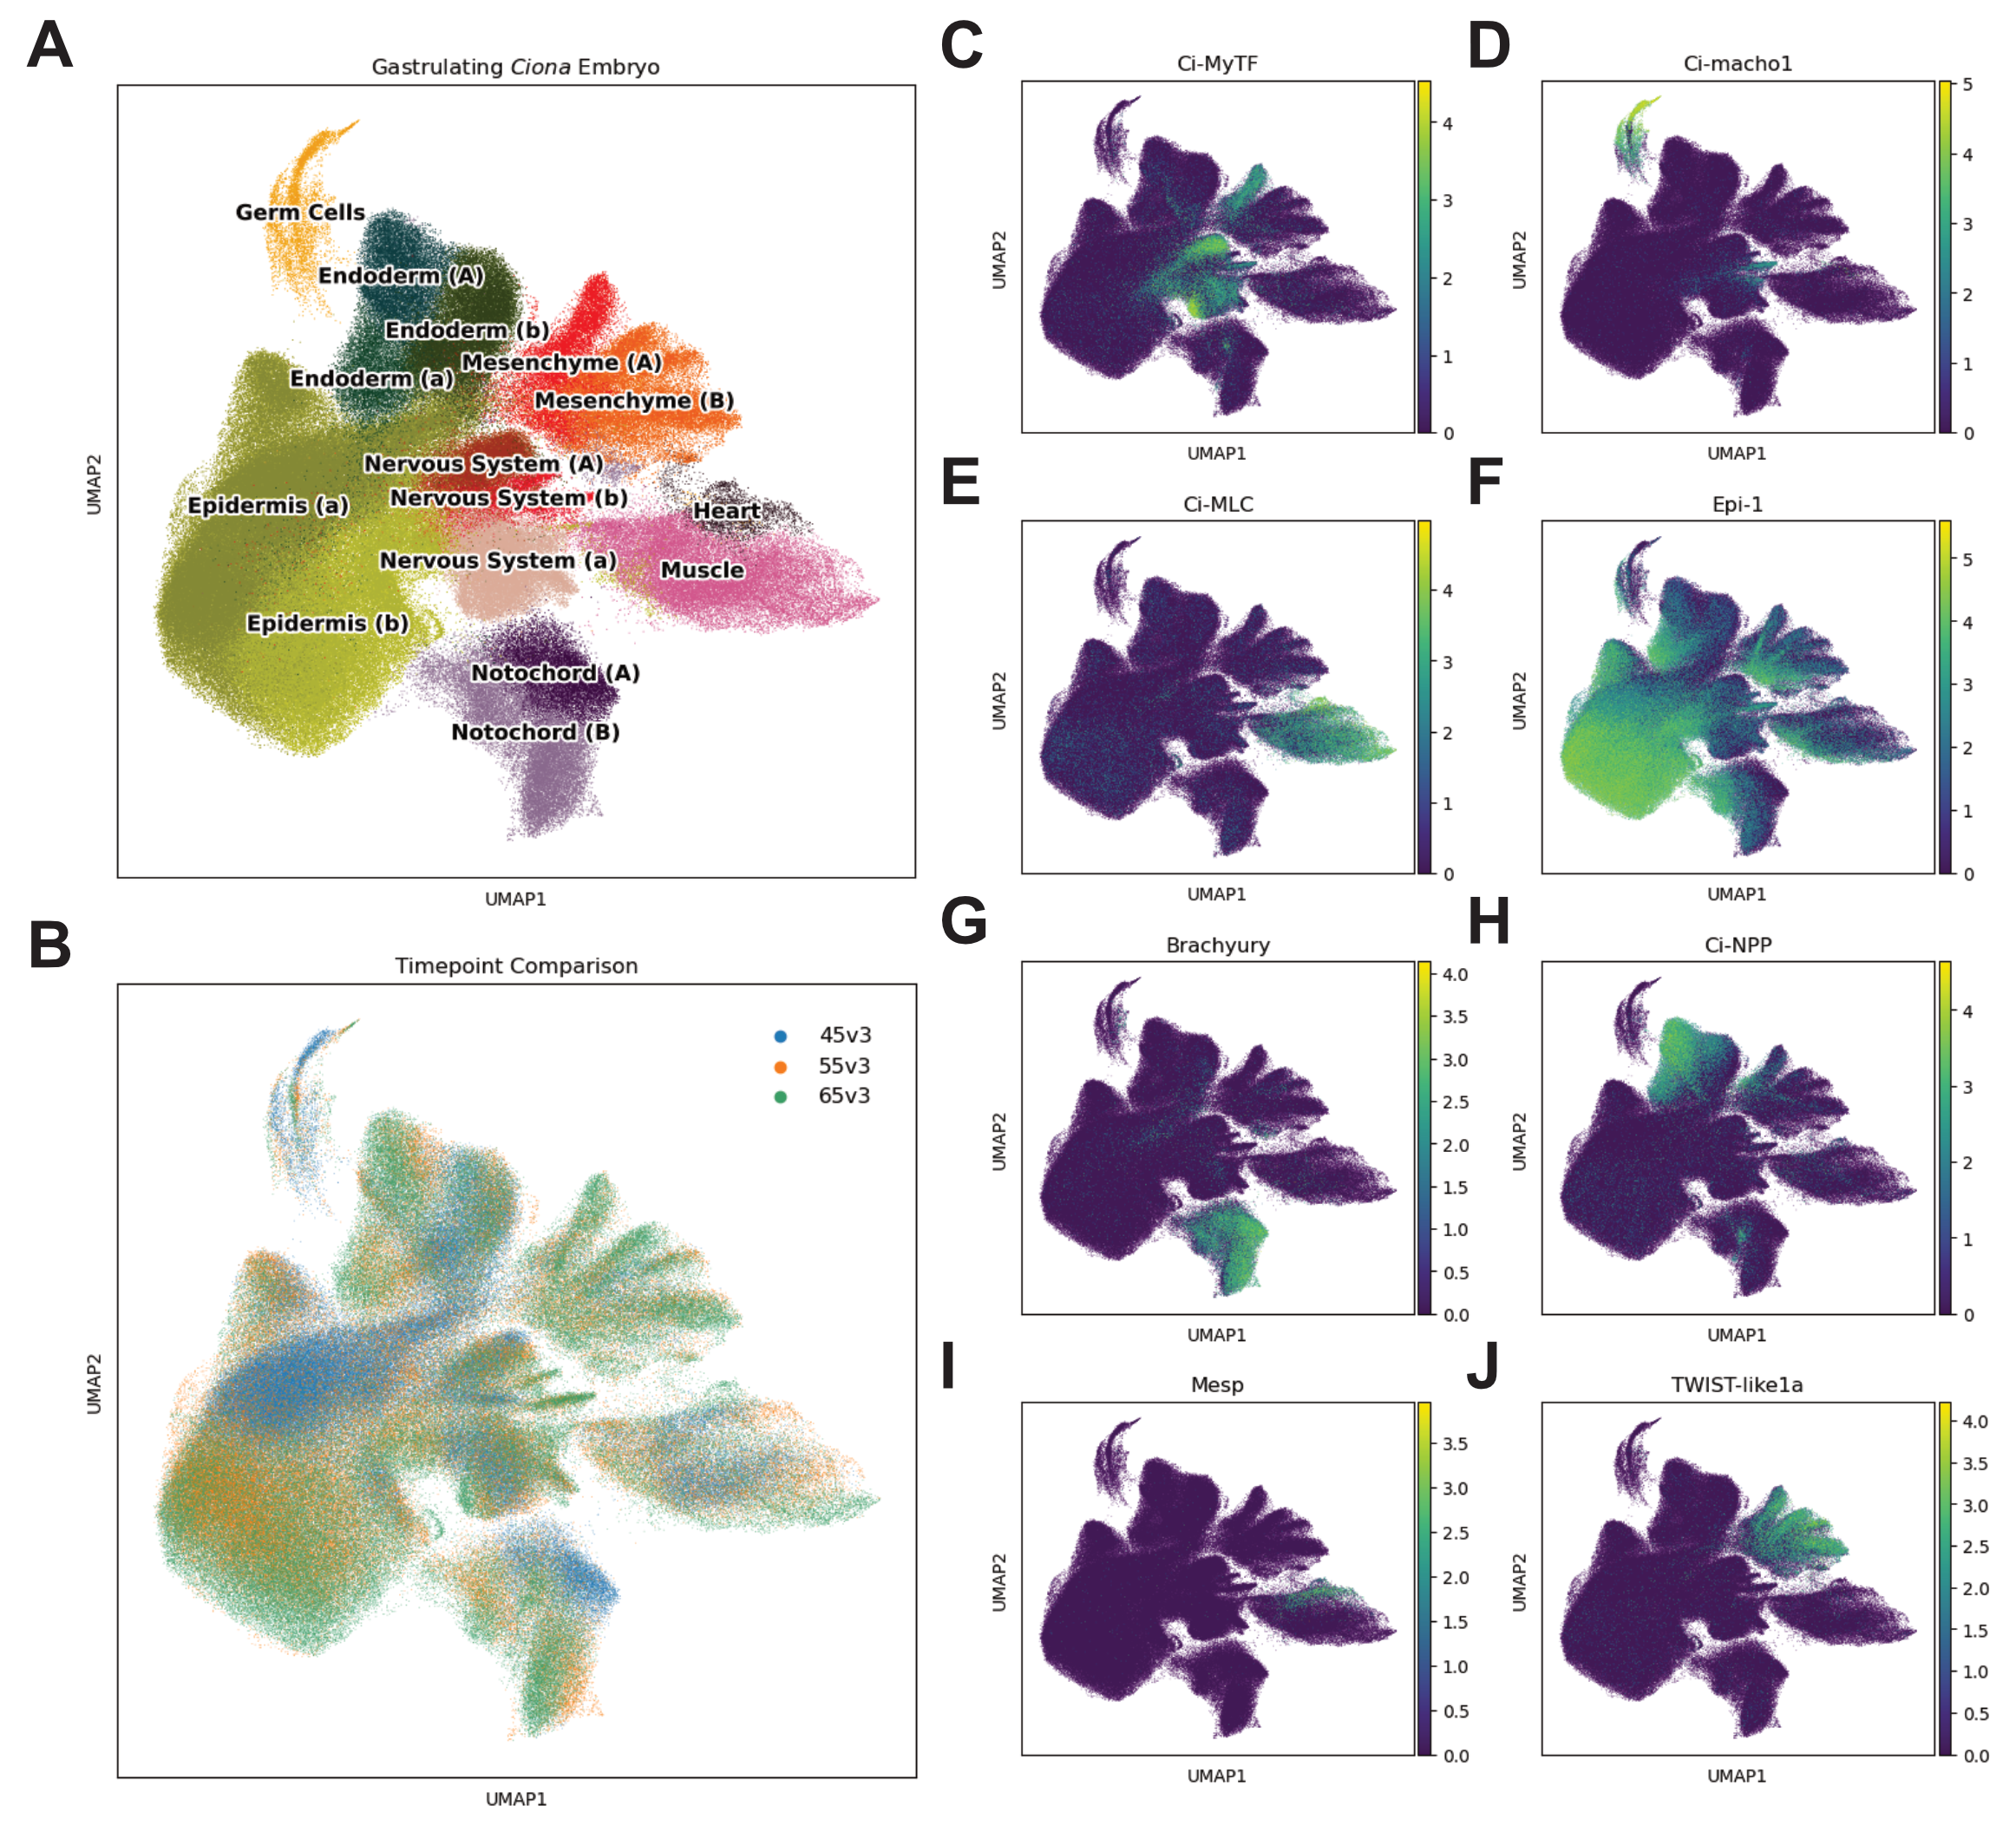
\includegraphics[scale=.8]{4_figures-and-files/Fig1_Single-Cell-Atlas-Clustering.png}
    \caption[Single-cell transcriptome atlas of the developing \textit{Ciona} gastrula]{\textbf{A.} UMAP plot of all cell types present during \textit{Ciona} gastrulation (consolidated across the 4.5 hpf, 5.5 hpf, and 6.5 hpf time points) resolved into the particular A, B, a, or b-lineages present in the \textit{Ciona} embryo at the 4-cell stage. The distribution of cells across major cell types can be found in Table \ref{tab:single-cell proportion of cells}. \textbf{B.} UMAP plot of cells in the \textit{Ciona} gastrula separated by time point, where \texttt{45v3} represents the 4.5 hpf time point, \texttt{55v3} the 5.5 hpf time point, and \texttt{65v3} the 6.5 hpf time point. \textbf{C-J.} UMAP visualizations of various canonical cell type marker genes used in the determination of cell type cluster identification.}
    \label{fig:1 single cell clustering}
\end{figure}

\begin{small}
    \begin{table}[ht]
        \centering
        \caption{Distribution of cells across annotated cell types} 
        \begin{tabular}{|p{.18\textwidth}|p{.15\textwidth}|p{.2\textwidth}|p{.2\textwidth}|}
            \hline
            % Define the table columns for the first and all subsequent pages
            \textbf{CELL TYPE} & \textbf{NUMBER OF CELLS} & \textbf{\% EMBRYO, DATA} & \textbf{\% EMBRYO, LITERATURE} \\ \hline 
            
            % Start table content
            %%%%% %%%%% %%%%% %%%%% %%%%% %%%%% %%%%% %%%%% %%%%% %%%%% %%%%% %%%%%
            Epidermis & 174,113 & 48.82	& - \\
            Endoderm & 44,816 & 12.57 & - \\
            Nervous System & 42,338 & 11.87 & 12.68 \\
            Mesenchyme & 31,695 & 8.89 & - \\
            Notochord & 31,263 & 8.77 & 6.67 \\
            Muscle & 24,661 & 6.91 & 5.33 \\
            Germ Cells & 4,730 & 1.33 & 0.67 \\
            Heart & 3,055 & 0.86 & 1.33 \\
            \hline
        \end{tabular}
        \label{tab:single-cell proportion of cells}
    \end{table}
\end{small}		

\subsection{Validating single-cell RNA-sequencing results with \textit{in situ} hybridization studies}

For some of the \textit{in situs} we found on the Aniseed database alongside canonical cell type markers, they were either dated, poor resolution, or had ambiguous expression patterns despite being marked as exclusively expressed within a certain cell type according to the Aniseed API \cite{dardaillon2020}. Thus, we sought to verify markers identified through our clustering methods using fluorescent \textit{in situ} hybridization (FISH) imaging performed in our lab (see Methods). As an example, we used \textit{Brachyury} to identify the notochord cluster in our UMAP visualization as it is known to be affiliated with notochord development in \textit{Ciona} (Figure \ref{fig:2 single cell notochord markers}) \cite{chesley1935,wilkinson1990,yasuo1993,reeves2021,casey1998,conlon2001,barnett1998,corbo1997,chiba2009,jose-edwards2015a,lolas2014,katikala2013,schulte-merker1995,muller1997,matsumoto2007a,passamaneck2009a}. After identifying the notochord cluster with \textit{Brachyury}, we found another marker, \textit{Orphan bHLH1} (Figure \ref{fig:2 single cell notochord markers}D), where it was unclear if it was also notochord-specific based on \textit{in situ} images on Aniseed. We then tested the two markers in tandem using FISH (Figure \ref{fig:2 single cell notochord markers}E-G), ultimately confirming their co-expression in the notochord and showing the validity of our single-cell clustering results. 

\begin{figure}[p]
    \centering
    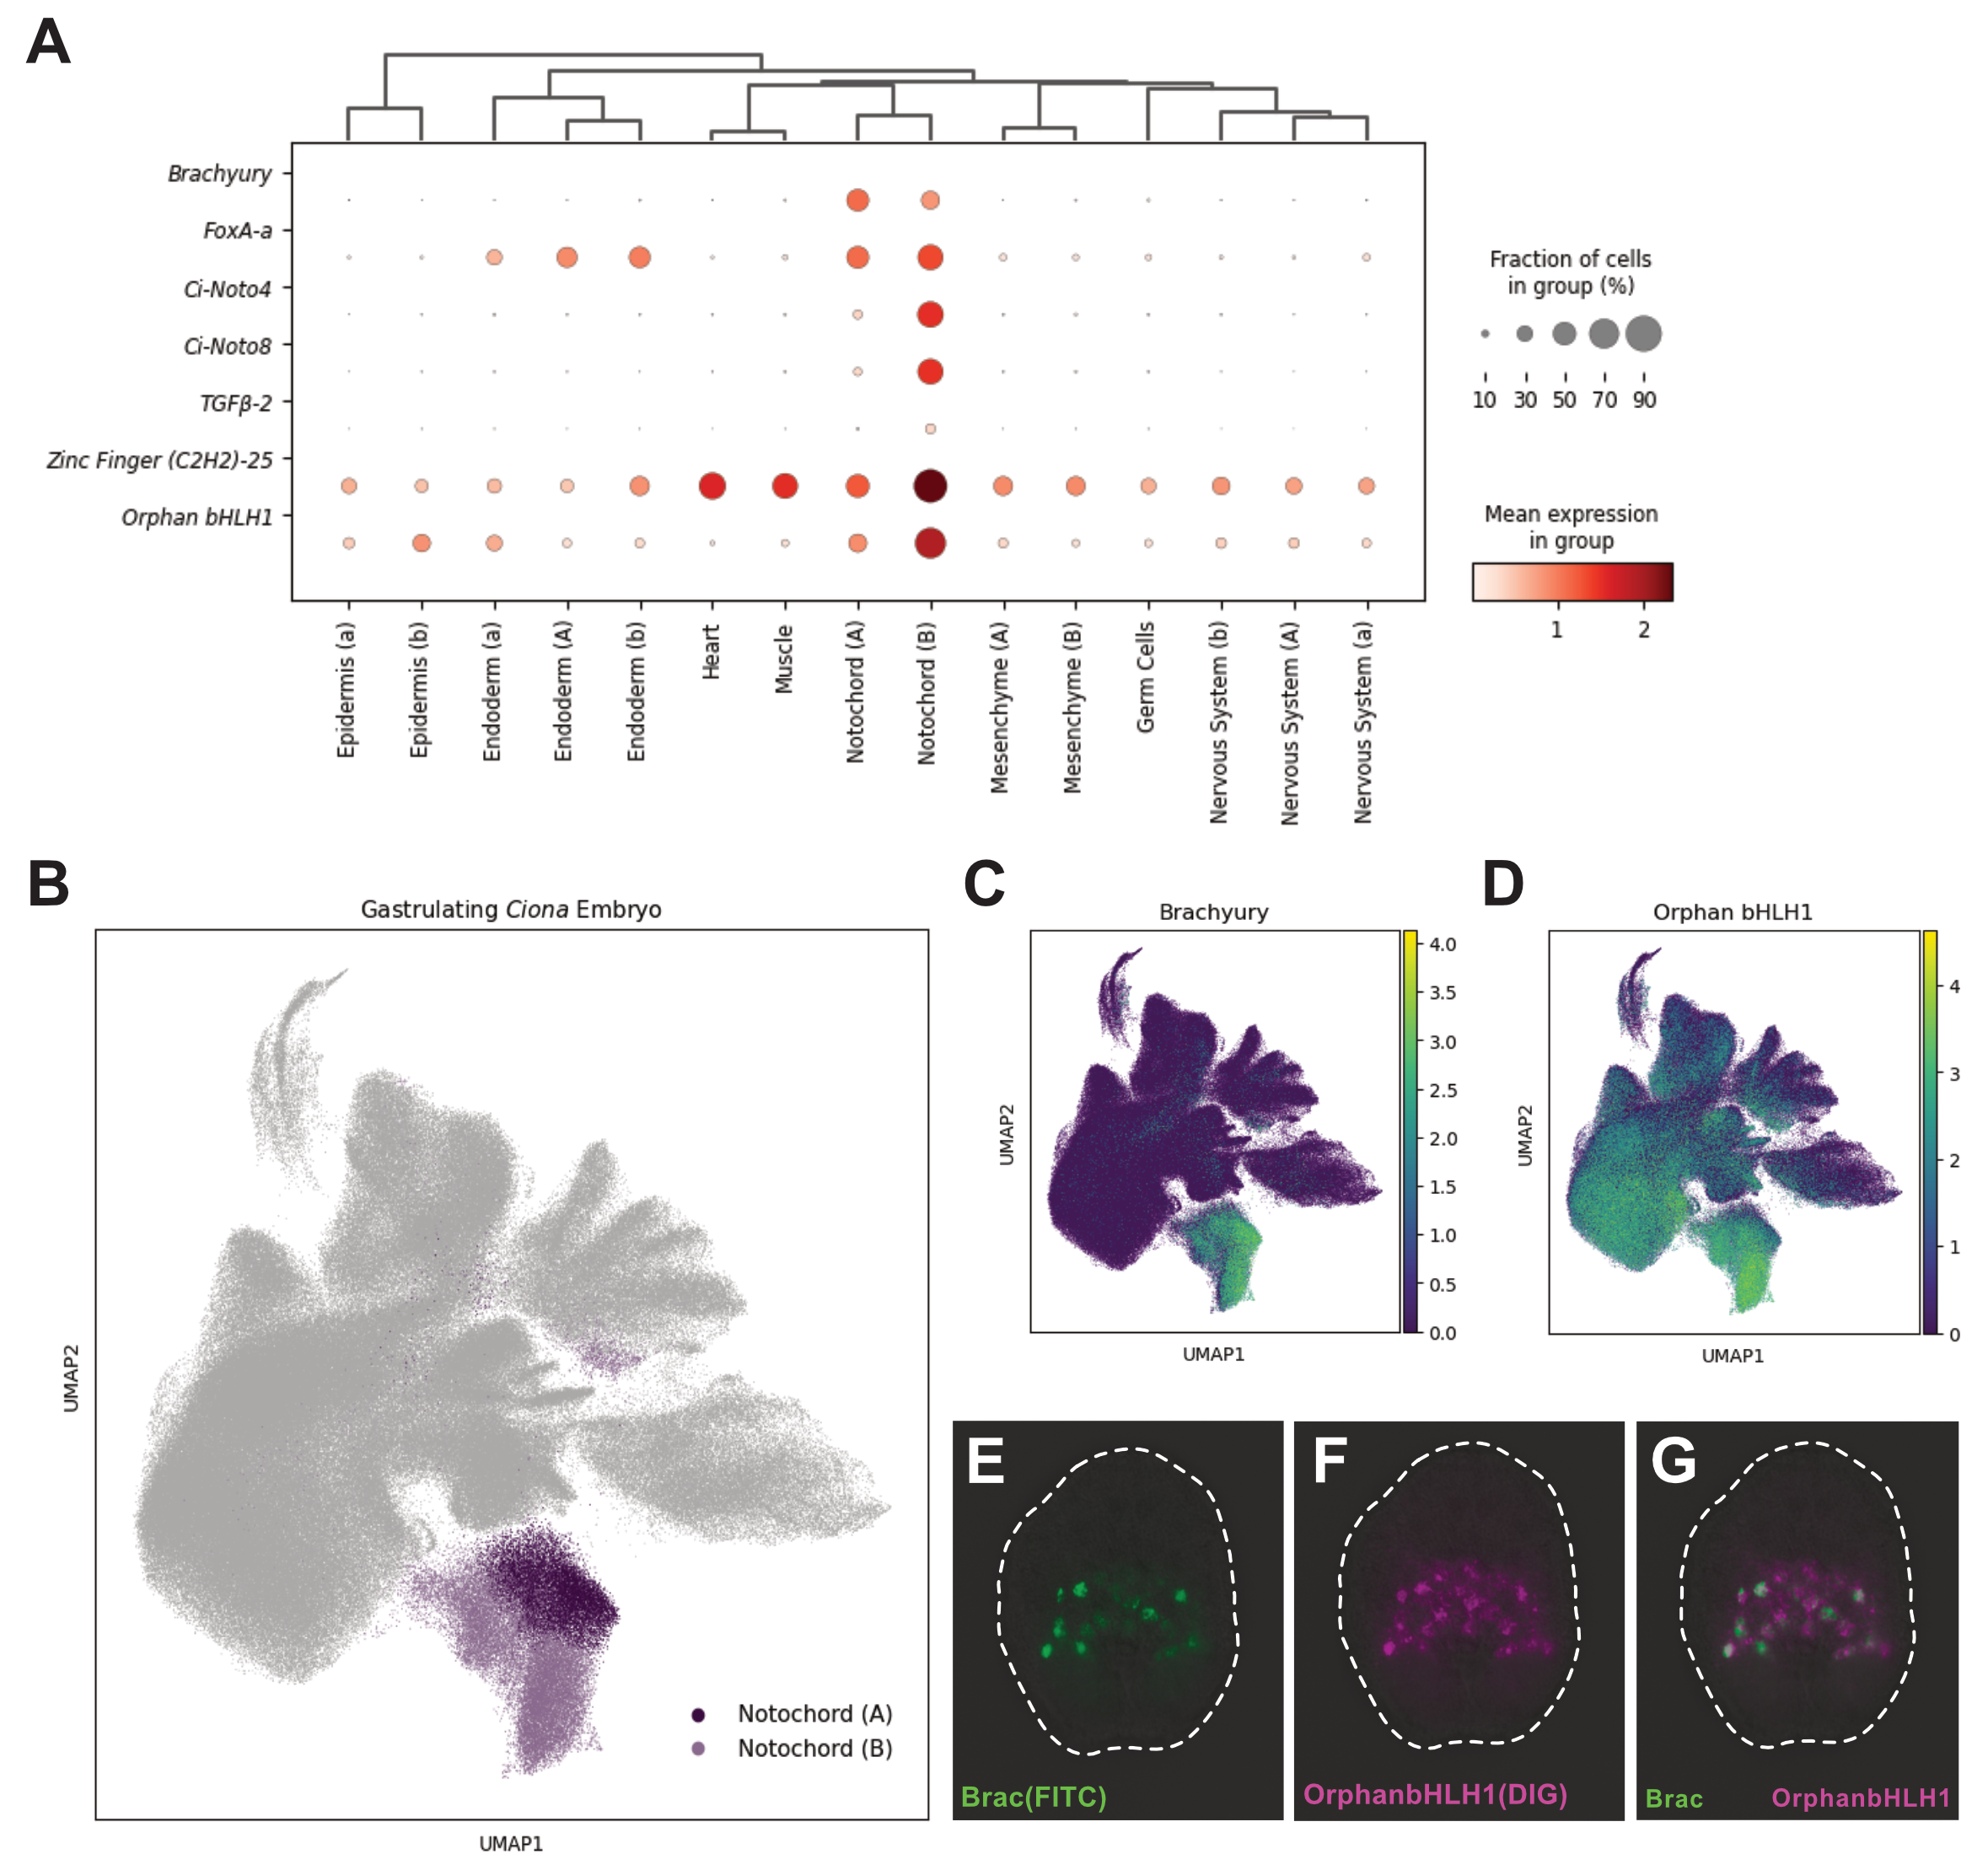
\includegraphics[scale=.8]{4_figures-and-files/Fig2_Notochord-Markers.png}
    \caption[Canonical \textit{Ciona} notochord markers \textit{Brachyury} and \textit{Orphan bHLH1} assist in validating cell clusters]{\textbf{A.} Dot plot of key notochord markers, including \textit{Brachyury}, \textit{FoxA-a}, \textit{Ci-Noto4}, \textit{Ci-Noto8}, \textit{TGF$\beta$-2}, and \textit{Zinc Finger (C2H2)-25}, in comparison to a less-studied notochord marker, \textit{Orphan bHLH1}. \textbf{B.} UMAP plot of cells in the \textit{Ciona} gastrula with the A-line and B-line notochord lineages highlighted in dark and light purple, respectively. \textbf{C-D.} UMAP visualizations of \textit{Brachyury} (C) and \textit{Orphan bHLH1} (D) in the single-cell atlas. \textbf{E-G.} \textit{FISH} images of \textit{Brachyury} (E), \textit{Orphan bHLH1} (F), and the overlay of the two (G) in 5.5 hpf \textit{Ciona} embryos (late gastrula stage).}
    \label{fig:2 single cell notochord markers}
\end{figure}

As expected from the high resolution of our study owing to the large number of cells encompassing each time point, we were also able to identify novel markers for particular cell types. One such marker, a \textit{Ciona} gene that had sequence homology to the vertebrate gene \textit{Arx}, was identified (Figure \ref{fig:3 single cell neural markers}). \textit{Ci-Arx} was found to be specifically expressed to the A-lineage nervous system of \textit{Ciona} corresponding to Row III and Row IV of the developing neural plate during gastrulation (Figure \ref{fig:3 single cell neural markers}A, Figure \ref{fig:3 single cell neural markers}D-G). These rows form the anterior sensory vesicle in \textit{Ciona} in the adult organism, correlating to the brain \cite{satoh2014}. Our data also corrobrates the finding of \textit{Ci-Arx} and its implications in the anterior sensory vesicle from the Cao \textit{et al.} (2019) single-cell study in \textit{Ciona} \cite{cao2019}. Previous literature has shown \textit{Arx} expression in the embryonic forebrain of both mouse and zebrafish and has implicated \textit{Arx} in X-linked lissencephaly, a human disease marked by the absence of folds in the cerebral cortex and an abnormally small head \cite{miura1997,miura1997,kitamura2002,lim2019,fulp2008}. Additionally, we found another marker within \textit{Ciona} that had sequence homology to vertebrate gene \textit{SWT1} and that was specifically expressed in the germ cells of the embryo (Figure \ref{fig:4 single cell germ cell markers}). While it is not characterized in \textit{Ciona}, the vertebrate \textit{Swt1} has been found in human testicular tissue \cite{fagerberg2014}. Additionally, vertebrate \textit{SWT1} is also relatively understudied within germ cells, providing a potential avenue for future research on its conservation and function. The discovery of \textit{Ci-SWT1} and \textit{Ci-Arx} from our single-cell map of the gastrulating \textit{Ciona} embryo represents a potential model for interrogation of novel gene expression patterns and hints at the potential usage of our atlas to uncover conserved genes delineating cell fate.

\begin{figure}[p]
    \centering
    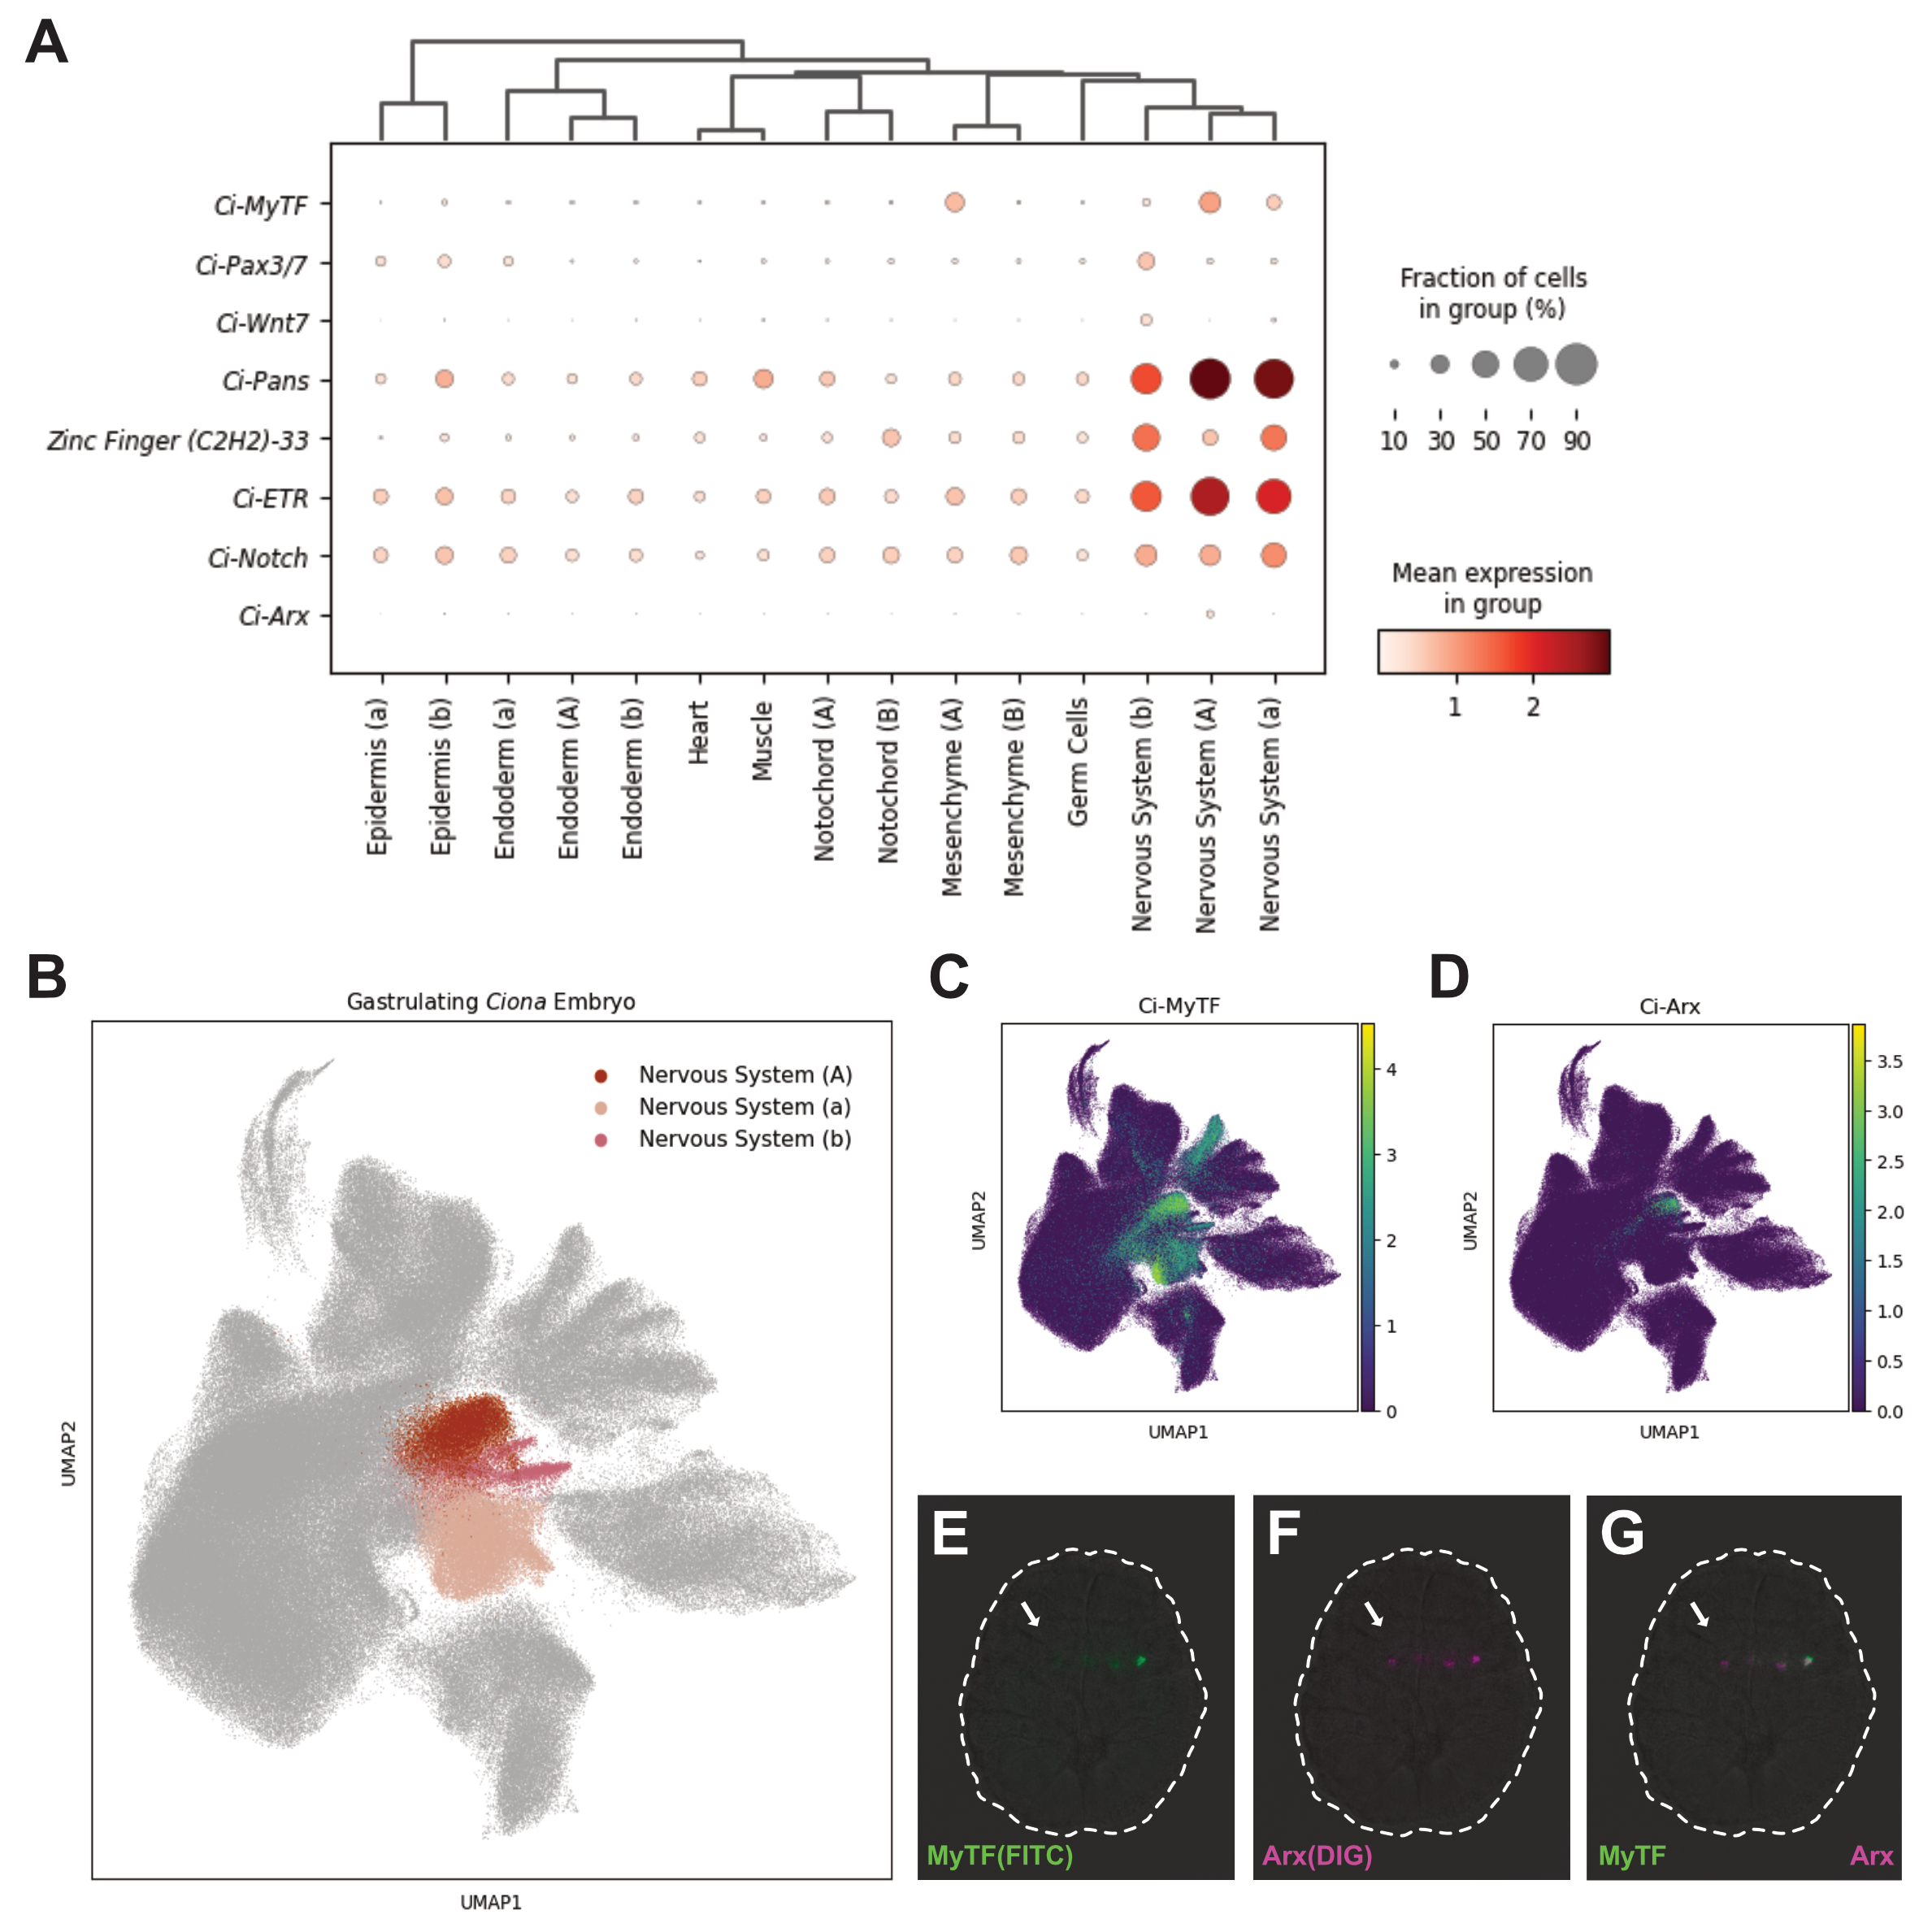
\includegraphics[scale=.7]{4_figures-and-files/Fig3_Arx-Neural-Markers.png}
    \caption[Vertebrate forebrain marker \textit{Arx} found in \textit{Ciona} A-line nervous system lineage]{\textbf{A.} Dot plot of key nervous system markers, including \textit{Ci-MyTF}, \textit{Ci-Pax3/7}, \textit{Ci-Wnt7}, \textit{Ci-Pans}, \textit{Zinc Finger (C2H2)-33}, \textit{Ci-ETR}, and \textit{Ci-Notch}, in comparison to a putative \textit{Ciona} neural marker, \textit{Ci-Arx}, as named via sequence homology. \textbf{B.} UMAP plot of cells in the \textit{Ciona} nervous system with the A-line, a-line, and b-line neural lineages highlighted in burnt orange, beige, and salmon respectively. \textbf{C-D.} UMAP visualizations of \textit{Ci-MyTF} (C) and \textit{Ci-Arx} (D) in the single-cell atlas. \textbf{E-G.} \textit{FISH} images of \textit{Ci-MyTF} (E), \textit{Ci-Arx} (F), and the overlay of the two (G) in 5.5 hpf \textit{Ciona} embryos (late gastrula stage). The arrow indicates the developing \textit{Ciona} neural plate Row III region of the embryo.}
    \label{fig:3 single cell neural markers}
\end{figure}

\begin{figure}[p]
    \centering
    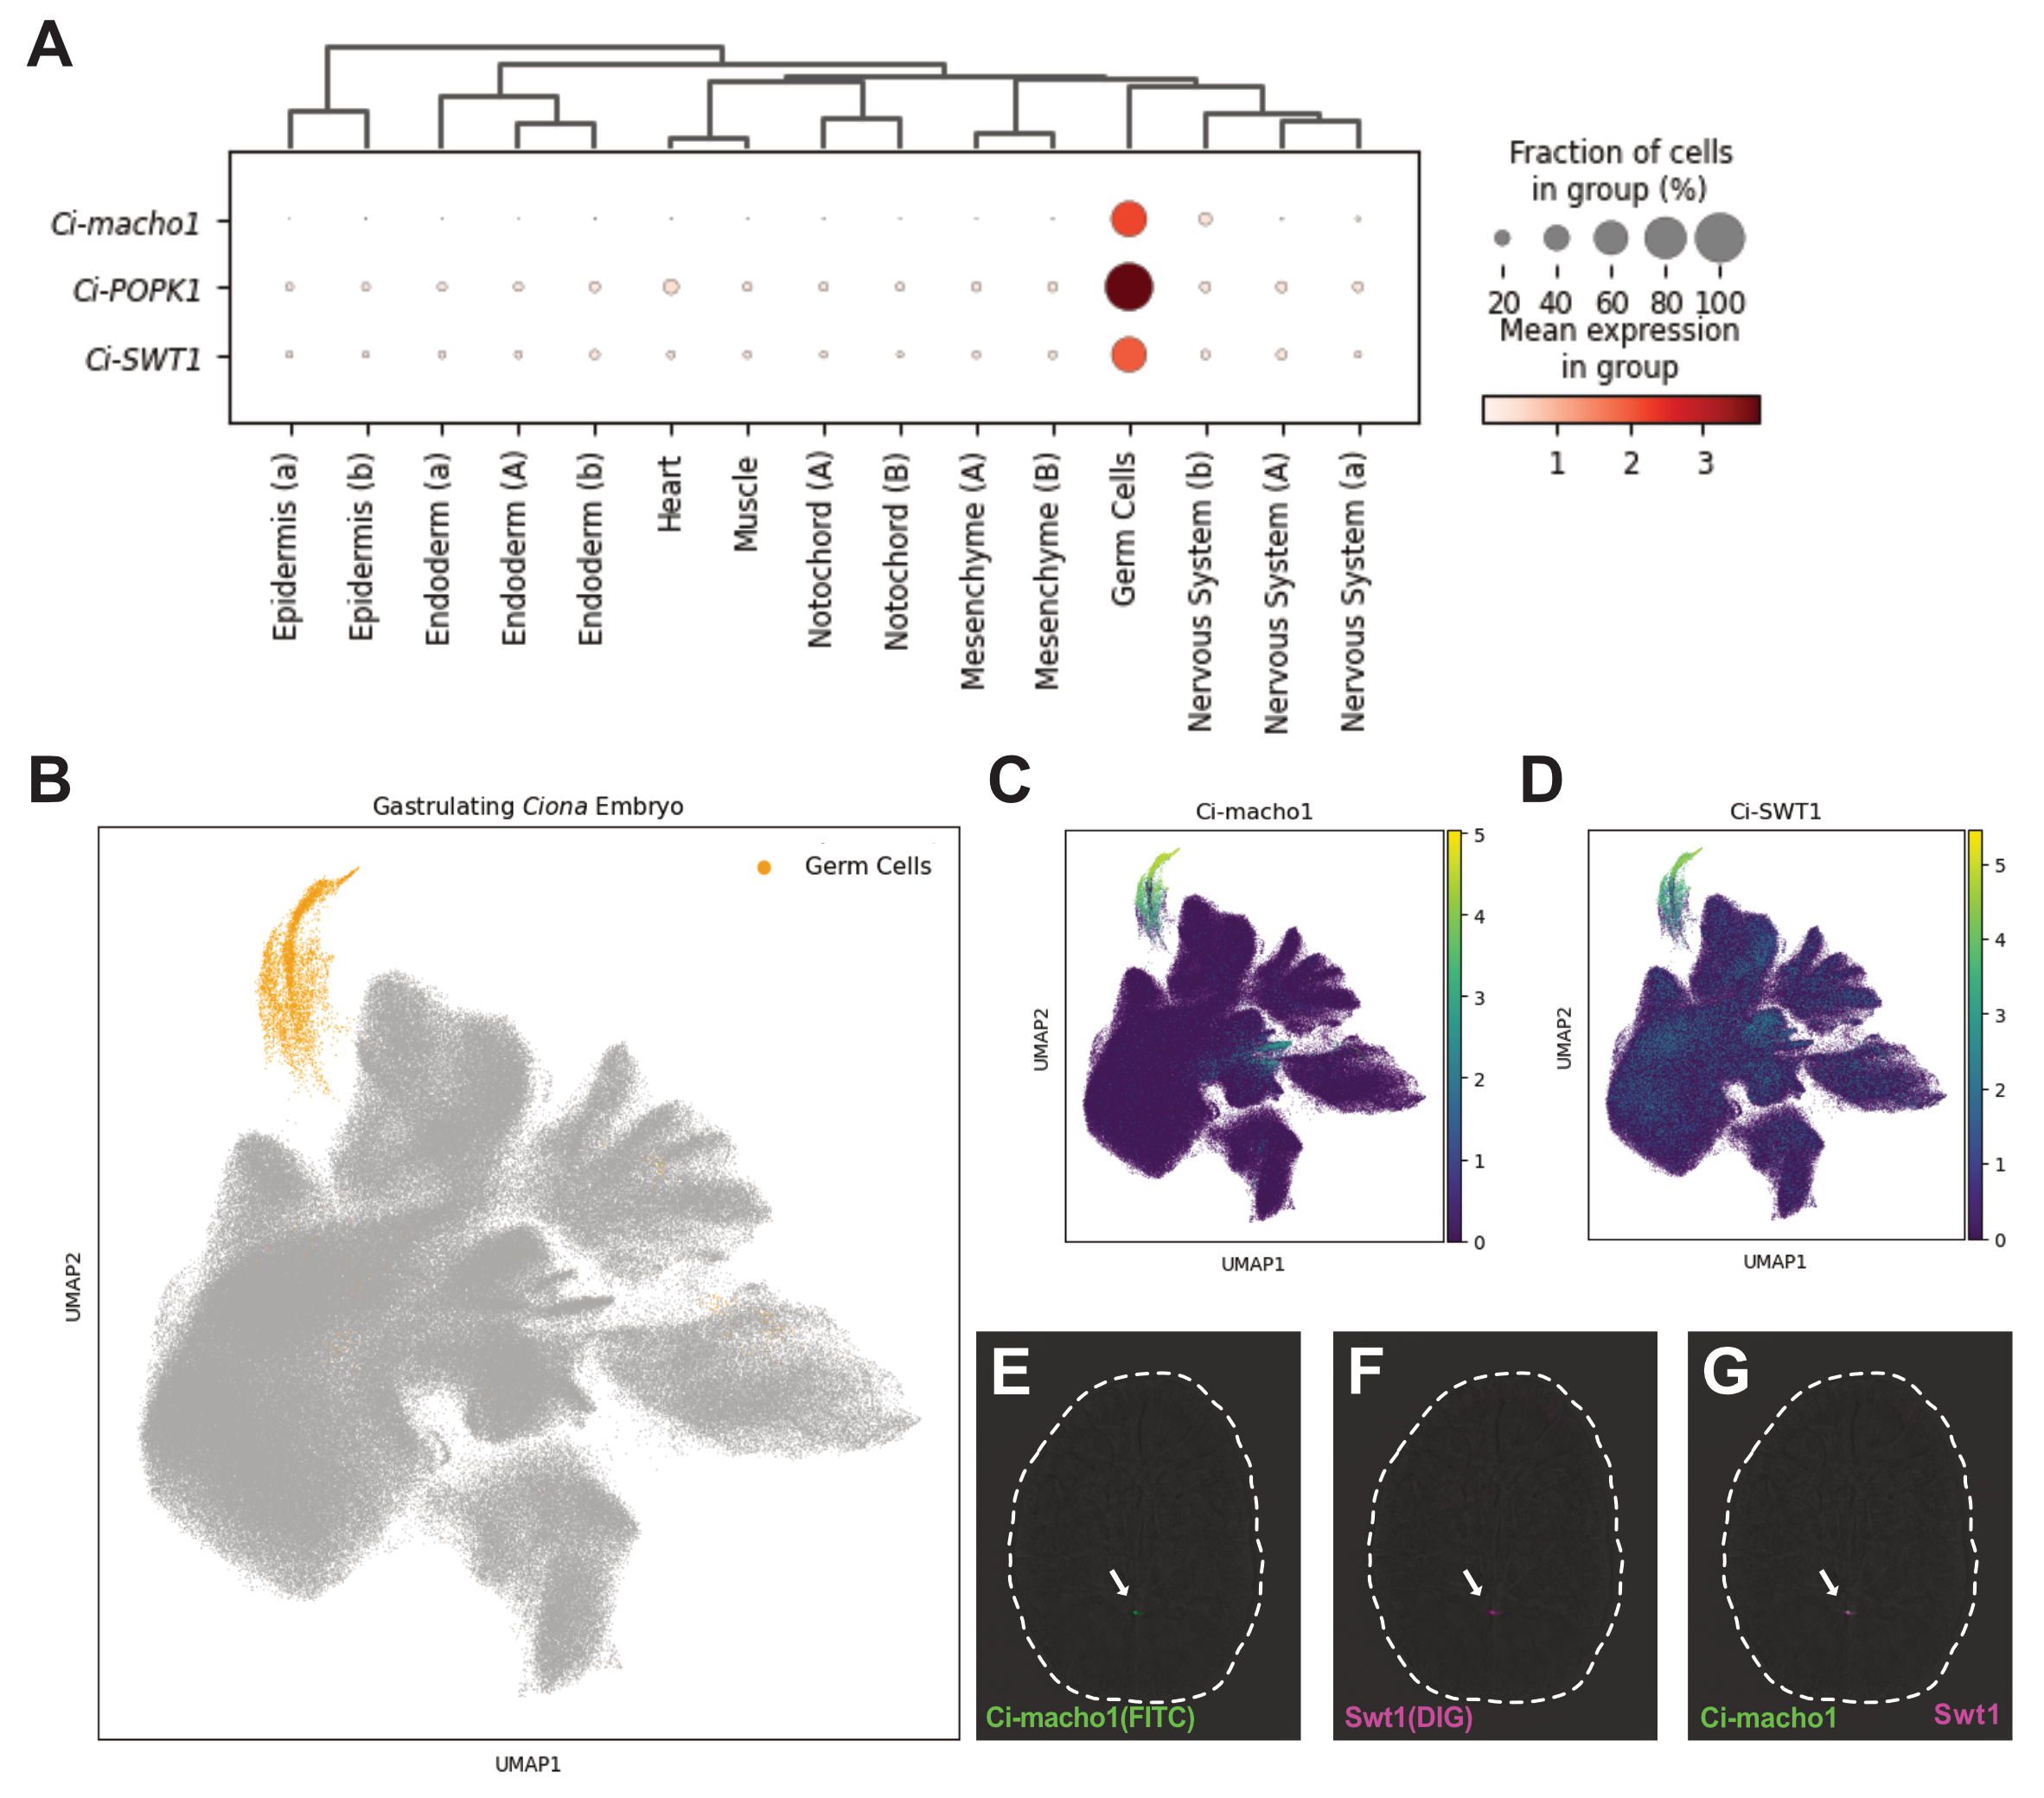
\includegraphics[scale=.7]{4_figures-and-files/Fig4_Swt1-Germ-Cell-Markers.png}
    \caption[Discovery of \textit{SWT1} found in the \textit{Ciona} germ cell cluster]{\textbf{A.} Dot plot of key germ cell markers, including \textit{Ci-macho1} and \textit{Ci-POPK1}, in comparison to a putative \textit{Ciona} germ cell marker, \textit{Ci-SWT1}, as named via sequence homology. \textbf{B.} UMAP plot of cells in the highly distinct \textit{Ciona} germ cell cluster in orange. \textbf{C-D.} UMAP visualizations of \textit{Ci-macho1} (C) and \textit{Ci-SWT1} (D) in the single-cell atlas. \textbf{E-G.} \textit{FISH} images of \textit{Ci-macho1} (E), \textit{Ci-SWT1} (F), and the overlay of the two (G) in 5.5 hpf \textit{Ciona} embryos (late gastrula stage). The arrow indicates the location of the \textit{Ciona} germ cells.}
    \label{fig:4 single cell germ cell markers}
\end{figure}

%%%%%%%%%%%%%%%%%%%%%%%%%%%%%%%%%%%%%%%%%%%%%%%%%%%%%%%%%%%%%%%%%%%%%%%%%%%%%%%%
\section{Discussion}
%%%%%%%%%%%%%%%%%%%%%%%%%%%%%%%%%%%%%%%%%%%%%%%%%%%%%%%%%%%%%%%%%%%%%%%%%%%%%%%%

Through scRNA-sequencing at whole embryos at a relatively small but expansive time frame of development, we were able to uncover the transcriptional signatures of major cell types in the \textit{Ciona} gastrula. While there are already a multitude of single-cell studies that have been performed, this study constitutes one of the highest resolution atlases to date, confirming results from the previous atlas-scale effort, but with a restricted time window. With the findings of well-studied, canonical markers within \textit{Ciona} to be specifically expressed within particular cell types alongside understudied genes, we hope that this dataset will provide suitable groundwork for future explorations into cell fate specification and its potential conservation across species \cite{winkley2021,sladitschek2020,zhang2020,ilsley2020,wang2019,horie2018,wang2021,cao2019}.

%%%%%%%%%%%%%%%%%%%%%%%%%%%%%%%%%%%%%%%%%%%%%%%%%%%%%%%%%%%%%%%%%%%%%%%%%%%%%%%%
\section{Materials and Methods}
%%%%%%%%%%%%%%%%%%%%%%%%%%%%%%%%%%%%%%%%%%%%%%%%%%%%%%%%%%%%%%%%%%%%%%%%%%%%%%%%

\subsection{\textit{Ciona} handling, collection, dissociation, and imaging of embryos}
Adult \textit{Ciona intestinalis type A}, also known as \textit{Ciona robusta}, were obtained from M-Rep and were maintained under constant illumination in seawater (obtained from Reliant Aquariums) at $18^\circ$C. \textit{Ciona} are hermaphroditic; therefore, there is only one possible sex for individuals. The age or developmental stage of the embryos studied is indicated in the main text.

\textit{Ciona} embryos were dechorionated as described in Christiaen \textit{et al.} (2009) \cite{christiaen2009}. Embryos were allowed to develop to either 4.5 hours post fertilization (hpf), 5.5 hpf, or 6.5 hpf in seawater. Embryos were dissociated by resuspension 1:3 Accumax:Artificial Seawater (ASW)-Mg-Ca, followed by light vortexing and gentle pipetting with Pasteur pipettes. Dissociated cells were washed twice with ASW + 0.1\% BSA and resuspended in 1 mL in ASW + 0.1\% BSA. Cells were strained through a 50 $\mu$m cell strainer, and cell concentration was counted on a hemacytometer. Fluorescent \textit{in situ} hybridization (FISH) assays were performed as previously described \cite{beh2007,ikuta2007,christiaen2009a,stolfi2014}. Embryos were counter-stained with DAPI (LifeTechnologies/Thermo Fisher Scientific, Waltham, MA). Images were taken using Leica Microsystems (Wetzlar, Germany) SP8 microscope.

\subsection{Single-cell RNA sequencing library construction, sequencing, data preprocessing, and preliminary clustering}
scRNA-seq was performed immediately after cell dissociation with the 10X Chromium 3' v2 kit (10X Genomics, Pleasanton, CA) following the manufacturer’s protocol. The target number of captured cells was 10,000 for each replicate of each time point. Sequencing libraries were prepared per the manufacturer’s protocol. Libraries were sequenced on the Illumina HiSeq 4000. Sequence alignment, filtering, barcode counting, and unique molecular identifier (UMI) counting were then performed using the cellranger (version 7.0.0) \verb|count| pipeline\footnote{\href{https://support.10xgenomics.com/single-cell-gene-expression/software/pipelines/latest/using/count}{https://support.10xgenomics.com/single-cell-gene-expression/software/pipelines/latest/using/count}} (10x Genomics, Pleasanton, CA) on each sample separately. We used the \textit{Ciona} HT genome assembly and KY gene models\footnote{\url{http://ghost.zool.kyoto-u.ac.jp/download_ht.html}} produced in 2019 and hosted on the Ghost database for this analysis \cite{satou2019}. The cellranger \verb|count| pipeline produced an RNA count matrix for each sample included in the study—three biological replicates across each of the 4.5 hpf, 5.5 hpf, and 6.5 hpf time points of \textit{Ciona} development. Using the Python software package scanpy (version 1.9.1) \cite{wolf2018}, all samples were combined into a single AnnData object for preprocessing. Across the three biological replicates of the 4.5 hpf, 5.5 hpf, and 6.5 hpf \textit{Ciona} embryos, there were 147,235 cells, 121,401 cells, and 157,661 cells, respectively. Before filtering, the RNA count matrix contained 426,297 cells x 18,788 genes. 

During preprocessing, doublet detection was performed using scanpy's external integration of the scrublet (version 0.2.3) tool to remove 10 cells from our RNA count matrix \cite{wolock2019}. Next, we performed the following steps in sequence to quality filter the data: we filtered out 56,539 cells that had less than 500 counts per cell, 41 cells that had more than 10,000 counts per cell, and finally, 13,216 cells that had less than 500 genes expressed. We then filtered out 2,307 genes detected in less than 20 cells. The resultant RNA count matrix contained 366,671 cells x 16,481 genes. Using the scanpy \verb|normalize_total()| method, we normalized all cells to represent 10,000 reads per cell, then logarithmized the data matrix using the scanpy \verb|log2p()| method. We then identified highly-variable genes using the dispersion-based method defined in scanpy, setting the minimum mean dispersion (\verb|min_mean parameter|) to 0.0125, the maximum mean dispersion (\verb|max_mean parameter|) to 3, and the minimum dispersion (\verb|min_disp parameter|) to 0.5. This approach identified 1,561 highly-variable genes to filter the data for downstream analysis. After regressing out the total number of counts per cell with the scanpy \verb|regress_out()| method, the data was scaled to unit variance with the scanpy \verb|scale()| method. We denoised the data using PCA as a dimensionality reduction method, then performed batch correction with scanpy's external integration of the harmonypy (version 0.0.5) tool \cite{slowikowski2022}. 

As a first step towards cell type clustering, we computed the neighborhood graph of cells using the PCA representation of the RNA count matrix using the scanpy \verb|neighbors()| method with a local neighborhood size of 10 and with 10 principal components. We embedded the graph into two-dimensional space using the uniform manifold approximation and projection (UMAP) dimension reduction technique for general non-linear dimensional reduction with the scanpy \verb|umap()| method. We performed UMAP as it is suggested by scanpy to be more faithful to the global connectivity of the manifold and, thus, better at preserving cellular trajectories. Finally, we directly clustered the neighborhood graph of cells in our data using the Leiden graph-clustering method implemented in the scanpy \verb|leiden()| method. In total, 36 clusters were found within our data. 

\subsection{Cell type cluster identification in the \textit{Ciona intestinalis} gastrulation atlas}
After performing Leiden clustering on our single-cell \textit{Ciona} gastrulation atlas, we annotated the clusters to correspond to tissue types present in the embryo. To expedite the clustering process, we leveraged the Aniseed API to access timepoint-specific gene location information extracted from user-submitted and published \textit{in situ} images \cite{dardaillon2020}. Currently, two gene models in circulation for \textit{Ciona} are hosted on the Ghost database: the KH model\footnote{\url{http://ghost.zool.kyoto-u.ac.jp/cgi-bin/gb2/gbrowse/kh/}} and the updated KY model\footnote{\url{http://ghost.zool.kyoto-u.ac.jp/default_ht.html}} \cite{dehal2002,satou2019,imai2004}. While Aniseed uses the KH models in their API, we generated our RNA count matrix with the KY gene model. As a first step, we translated the 1,561 KY gene identifiers in our RNA count matrix to KH identifiers using a chromosomal distance-based Python script (\url{https://github.com/katarzynampiekarz/ciona_gene_model_converter}). This allowed us to integrate Aniseed's gene location information at our time points of interest with our RNA count matrix to expedite the identification of cell-type clusters during gastrulation. 

For the clustering applied to UMAP coordinates of the whole dataset, we refined annotation results by first comparing the expression pattern of top marker genes and known \textit{Ciona} regulatory genes between the Leiden clusters. Clusters with similar expression patterns to key regulatory genes and known markers were considered the same cell type. We also compared our annotation results with the \textit{in situ} records accessed via that Aniseed API or by viewing the \textit{in situ} images recorded in the Ghost and Aniseed databases. We carefully checked the gene expression pattern for putative newly discovered cell types in clusters with poorly annotated marker genes to ensure no ambiguous expression of known markers. We identified 15 clusters representing various lineages of the following cell types: endoderm, epidermis, germ cells, heart, mesenchyme, muscle, nervous system, and notochord.

%%%%%%%%%%%%%%%%%%%%%%%%%%%%%%%%%%%%%%%%%%%%%%%%%%%%%%%%%%%%%%%%%%%%%%%%%%%%%%%%
\section{Acknowledgements}
%%%%%%%%%%%%%%%%%%%%%%%%%%%%%%%%%%%%%%%%%%%%%%%%%%%%%%%%%%%%%%%%%%%%%%%%%%%%%%%%

This work would not have been possible without the help of the following individuals that were fundamental to the execution of this project: Benjamin P. Song, Hannah Finnegan, and Emma K. Farley. I would also like to thank the Farley Lab for helpful discussions during the analysis of the data included in this work, especially with regards to cell cluster identification and imaging of cell type markers. I would also like to thank the UCSD IGM Genomics Center for their assistance with sequencing. Finally, I would also like to thank Alberto Stolfi and Katarzyna Piekarz from the Georgia Institute of Technology for their generous support in providing a script to translate between the \textit{Ciona intestinalis} KH gene identifiers and the updated KY gene identifiers. Their assistance was fundamental to the identification of cell-type clusters in this work.

%%%%%%%%%%%%%%%%%%%%%%%%%%%%%%%%%%%%%%%%%%%%%%%%%%%%%%%%%%%%%%%%%%%%%%%%%%%%%%%%
\section{Footnotes}
%%%%%%%%%%%%%%%%%%%%%%%%%%%%%%%%%%%%%%%%%%%%%%%%%%%%%%%%%%%%%%%%%%%%%%%%%%%%%%%%

\subsection{Author contributions}
E.K.F., B.P.S., M.F.R, designed experiments. B.P.S. and H.F. conducted experiments. M.F.R. conducted bioinformatic analyses. M.F.R. wrote the chapter. E.K.F., M.F.R., and B.P.S. were involved in editing the chapter. 

\subsection{Funding}
M.F.R. was supported by NIH T32 GM008666. B.P.S. was supported by NIH T32 GM133351. E.K.F., M.F.R., B.P.S., and H.F. were supported by NIH DP2HG010013.

\subsection{Data availability}
Further information and requests for resources and reagents should be directed to and will be fulfilled by the lead contact, Emma K. Farley (efarley@ucsd.edu), upon request. All FASTQ files and annotated scanpy \verb|AnnData| objects will be deposited to GEO when a publication is made available. All original code for this chapter has been deposited to GitHub (\url{https://github.com/mragsac/Ciona-Single-Cell-Gastrulation-Study}) and will be made publicly available. Any additional information or data required to recapitulate the study reported in this chapter is available upon request.

\subsection{Declaration of interests}
The authors declare no competing interests.
